\section{Untapped enormous potential: integrating mobile devices into the Grid}
Now, with general understanding of what Grid Computing is and how mobile devices evolved over the years, the main topic of this work can be discussed: integrating (using volunteer computing) mobile devices into Grid Computing alongside desktop computers exploiting an enormous quantity of computational resources that lay unused in the pockets of billions of users.

\subsection{Idea: strength in numbers}
As seen in \textit{figure \ref{fig:global_sales_of_pcs_and_smartphones}}, the market has an enormous number of smartphones sold, thus resulting in an abundance of available devices that billions of users use every day (tablets have also to be taken in consideration).
\vspace{10mm}

\begin{figure}[!ht]
    \centering
    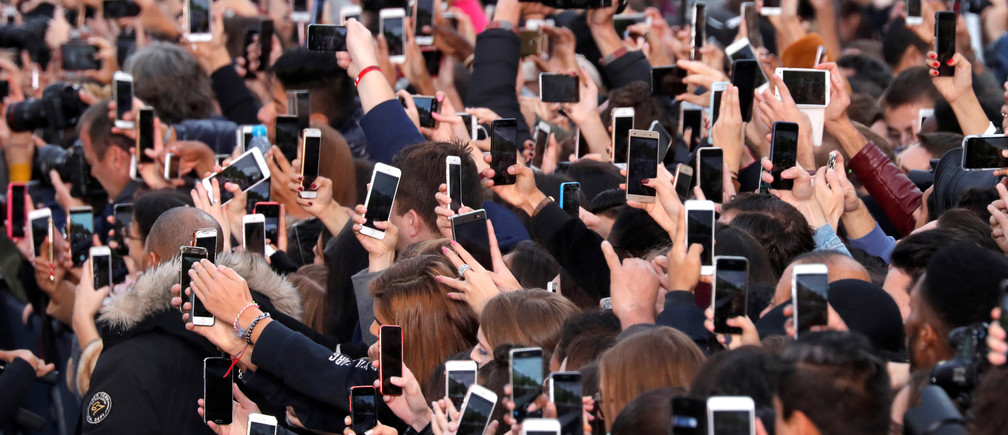
\includegraphics[scale=1.35]{document/chapters/chapter_1/images/people_using_smartphones.jpg}
    \caption{Mobile devices (smartphones in particular) are now an overly available commodity that is used daily on a regular basis}
    \label{fig:people_using_smartphones}
\end{figure}

Despite smartphones and tablets are not on the same level (in terms of hardware capabilities) with current computers, it is possible to exploit the availability of a vast number of devices as a leverage to compensate the performances of such mobile devices.
This concept becomes increasingly relevant also considering the tendency of users to progressively use less and less desktop computers in favor of their mobile devices.

\subsection{Previous works and how limitations evolved}
TODO

\subsubsection{Mobile devices competitive performances}
TODO

\subsubsection{Mobile users common behavior}
TODO

\subsubsection{Economically sustainable internet connections}
TODO

\subsubsection{Standardized mobile market}
TODO

\subsubsection{Not only mobile: devices transparency principle}
TODO
